\documentclass[11pt,a4paper]{article}
\usepackage[T1]{fontenc}
\usepackage[utf8]{inputenc}
\usepackage[margin=2.5cm]{geometry}
\usepackage{amsmath,amssymb,amsthm}
\usepackage{graphicx}
\usepackage[hidelinks]{hyperref}
\usepackage{tikz}
\usetikzlibrary{3d}

\title{Continuity of Convex Functions on $\mathbb{R}^n$}
\author{Luigi de Alfaro}
\date{January 2025}

\begin{document}
\maketitle

\section{Introduction}

This note proves that a convex function $f : \mathbb{R}^n \to \mathbb{R}$ is
continuous everywhere. The result is classical. The usual argument invokes the
fact that a cube is the convex hull of its $2^n$ vertices, and then applies
Jensen's inequality in several variables.

I wrote this while in \emph{classes préparatoires}, where convex functions of
several variables and the multivariable form of Jensen's inequality are outside
the syllabus. The argument below therefore uses nothing beyond the two-point
definition of convexity. It builds a chain of $n$ inequalities, each one pinning
a further coordinate to $\pm 1$, until the point reaches a vertex of the
hypercube. The idea arose while exploring how convex functions of one variable
generalise to several dimensions.

One remark on which hypothesis does the work. The bounding argument of
Section~\ref{sec:bounding} only ever uses
$f(\lambda a + (1-\lambda) b) \le \max\big(f(a), f(b)\big)$, that is
quasiconvexity. Full convexity is needed only in Section~\ref{sec:contradiction},
where the slopes of a one-dimensional restriction are compared.

\section{Preliminaries}

Let $f : \mathbb{R}^n \to \mathbb{R}$ be a convex function. Recall that $f$ is
convex if for all $x, y \in \mathbb{R}^n$ and $\lambda \in [0,1]$:
\[
  f(\lambda x + (1-\lambda) y) \le \lambda f(x) + (1-\lambda) f(y).
\]
We aim to prove that $f$ is continuous everywhere in $\mathbb{R}^n$.

To do this, we use the following construction.

\begin{itemize}
  \item We define the unit sphere $S$ in the Euclidean norm $\|\cdot\|_2$ as
  \[
    S = \{ x \in \mathbb{R}^n : \|x\|_2 = 1 \}.
  \]
  \item We construct a hypercube containing $S$ by introducing the supremum norm
  \[
    \|x\|_\infty = \max(|x_1|, |x_2|, \dots, |x_n|).
  \]
  \item The unit sphere in this norm is the boundary of an $n$-dimensional
  hypercube centred at $0$, with vertices where each coordinate is $\pm 1$. In
  this context we are only interested in the boundary of the hypercube. We
  therefore define $H$ as the set of points satisfying $\|x\|_\infty = 1$, which
  ensures that at least one coordinate of $x$ reaches $\pm 1$.
\end{itemize}

\section{Proof of Continuity}

\subsection{Reduction by Contradiction}

Assume, for the sake of contradiction, that $f$ is not continuous at some point
$x_0 \in \mathbb{R}^n$. We may consider the function $x \mapsto f(x + x_0)$, so
we can assume $x_0 = 0$. By definition, there exists $\varepsilon > 0$ such that
for any $\delta > 0$ we can find $x \in B(0, \delta)$ satisfying
\[
  |f(x) - f(0)| \ge \varepsilon .
\]

We first show that $f(S)$ is bounded above. This will contradict the assumption
of discontinuity, as shown in the last part of the proof.

\subsection{Recursive Bounding of \texorpdfstring{$f(S)$}{f(S)}}
\label{sec:bounding}

We now present the recursive argument bounding $f(S)$. Define the boundary of
the hypercube $H$ as
\[
  H = \{ x \in \mathbb{R}^n : \|x\|_\infty = 1 \},
\]
and let $V(H)$ denote its vertices, the points where all $n$ coordinates are
equal to $\pm 1$. Let $z \in S$ be a point on the unit sphere; since
$\|z\|_\infty \le \|z\|_2 = 1$, the point $z$ lies in the closed cube
$[-1,1]^n$. The argument constructs a sequence of points $y_k$ such that $f(z)$
is bounded by the maximum of $f$ evaluated at the vertices of the hypercube, or
at $f(y_k)$. The recursion stops when $y_k$ becomes a vertex of the hypercube.

\begin{figure}[h!]
\centering
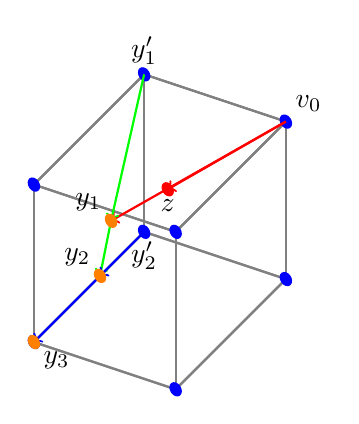
\begin{tikzpicture}[x={(0.9cm,-0.3cm)}, y={(0cm,1cm)}, z={(0.7cm,0.7cm)}, scale=2]

    % Edges of the hypercube
    \foreach \x in {0,1} {
        \foreach \y in {0,1} {
            \foreach \z in {0,1} {
                \draw[gray, thick] (\x, \y, 0) -- (\x, \y, 1);
                \draw[gray, thick] (\x, 0, \z) -- (\x, 1, \z);
                \draw[gray, thick] (0, \y, \z) -- (1, \y, \z);
            }
        }
    }

    % Vertices of the hypercube
    \foreach \x in {0,1} {
        \foreach \y in {0,1} {
            \foreach \z in {0,1} {
                \filldraw[blue] (\x, \y, \z) circle (0.04);
            }
        }
    }

    \coordinate (v0)  at (1,1,1);      % starting vertex
    \coordinate (vp1) at (0,1,1);      % vertex y'_1
    \coordinate (vp2) at (0,0,1);      % vertex y'_2
    \coordinate (z)   at (0.4,0.6,0.7);
    \coordinate (y1)  at (0,0.28,0.7);
    \coordinate (y2)  at (0,0,0.6);
    \coordinate (y3)  at (0,0,0);

    % Trajectory of the points y_k
    \draw[red,   thick, ->] (v0)  -- (z);
    \draw[red,   thick, ->] (v0)  -- (y1);
    \draw[green, thick, ->] (vp1) -- (y1);
    \draw[green, thick, ->] (y1)  -- (y2);
    \draw[blue,  thick, ->] (vp2) -- (y2);
    \draw[blue,  thick, ->] (y2)  -- (y3);

    \filldraw[red]    (z)  circle (0.04);
    \filldraw[orange] (y1) circle (0.04);
    \filldraw[orange] (y2) circle (0.04);
    \filldraw[orange] (y3) circle (0.04);

    \node[anchor=north]      at (z)   {\(z\)};
    \node[anchor=south west] at (v0)  {\(v_0\)};
    \node[anchor=south east] at (y1)  {\(y_1\)};
    \node[anchor=south east] at (y2)  {\(y_2\)};
    \node[anchor=north west] at (y3)  {\(y_3\)};
    \node[anchor=south]      at (vp1) {\(y'_1\)};
    \node[anchor=north]      at (vp2) {\(y'_2\)};

\end{tikzpicture}
\caption{The hypercube $H$ for $n = 3$ and the progression of the points $y_k$
starting from $z$. Here $y_1$ lies on a face, $y_2$ on an edge, and $y_3$ is a
vertex. At each step, $y'_k$ denotes the vertex obtained from $y_k$ by setting
every coordinate not yet equal to $\pm 1$ to the value $1$.}
\label{fig:hypercube}
\end{figure}

\paragraph{Step 1: setting.}
We aim to construct a sequence of points $y_k$ such that
\begin{itemize}
  \item at least $k$ coordinates of $y_k$ are equal to $\pm 1$,
  \item $\|y_k\|_\infty = 1$,
  \item $f(z) \le \max\left( \max_{v \in V(H)} f(v),\ f(y_k) \right)$.
\end{itemize}

\paragraph{Step 2: base case ($k = 1$).}
Start by constructing the line passing through the vertex
$v_0 = (1, 1, \dots, 1)$ and $z$. This line is parameterised as
\[
  \gamma(t) = v_0 + t (z - v_0), \qquad t \in \mathbb{R}.
\]
In terms of coordinates, the $i$-th coordinate of $\gamma(t)$ is
\[
  \gamma(t)_i = 1 + t(z_i - 1), \qquad i = 1, \dots, n.
\]
A coordinate with $z_i = 1$ is constant along $\gamma$ and already equal to
$\pm 1$, so we restrict attention to
\[
  I = \{\, i : z_i \neq 1 \,\}.
\]
This set is non-empty: if it were empty we would have $z = v_0$ and hence
$\|z\|_2 = \sqrt{n} > 1$ for $n \ge 2$, while for $n = 1$ the sphere consists of
the two vertices $\pm 1$ and there is nothing to prove.

For $i \in I$ the map $t \mapsto \gamma(t)_i$ is continuous, strictly monotone
and unbounded, and $\gamma(1)_i = z_i \in [-1,1]$. By the intermediate value
theorem there is therefore a unique $t'_i \ge 1$ with $\gamma(t'_i)_i = \pm 1$.
Define
\[
  t_1 = \min_{i \in I} t'_i .
\]
This choice ensures that the point $y_1 = \gamma(t_1)$ remains on the boundary
of the hypercube $H$: the smallest $t'_i$ guarantees that at least one
coordinate of $y_1$ reaches $\pm 1$ without the other coordinates exceeding the
bounds imposed by $H$. By construction,
\begin{itemize}
  \item $y_1$ has at least one coordinate equal to $\pm 1$,
  \item $\|y_1\|_\infty = 1$.
\end{itemize}
Note that, because $t_1 \ge 1$, we have $z = \gamma(1) \in [v_0, y_1]$. By
convexity of $f$,
\[
  f(z) \le \max\big( f(v_0), f(y_1) \big).
\]
This establishes the base case.

\paragraph{Step 3: inductive hypothesis.}
Assume that for some $k \ge 1$ there exists a point $y_k \in H$ such that
\begin{itemize}
  \item at least $k$ coordinates of $y_k$ are equal to $\pm 1$,
  \item $\|y_k\|_\infty = 1$,
  \item $f(z) \le \max\left( \max_{v \in V(H)} f(v),\ f(y_k) \right)$.
\end{itemize}

\paragraph{Step 4: inductive step ($k \to k+1$).}
If $y_k$ already has $n$ coordinates equal to $\pm 1$, then $y_k$ is a vertex of
$H$ and the proof is complete. Otherwise the set
\[
  J = \{\, i : y_k[i] \notin \{-1, 1\} \,\}
\]
is non-empty. Define $y'_k$ by fixing to $1$ all coordinates of $y_k$ indexed by
$J$, and keeping the other coordinates unchanged. Thus $y'_k$ is a vertex of $H$
agreeing with $y_k$ on every coordinate already equal to $\pm 1$. Construct the
line passing through $y'_k$ and $y_k$, parameterised as
\[
  \gamma(t) = y'_k + t (y_k - y'_k), \qquad t \in \mathbb{R}.
\]
In terms of coordinates, the $i$-th coordinate of $\gamma(t)$ is
\[
  \gamma(t)_i =
  \begin{cases}
    y_k[i], & i \notin J, \\[2pt]
    1 + t\,(y_k[i] - 1), & i \in J.
  \end{cases}
\]
The coordinates outside $J$ are constant along $\gamma$ and remain equal to
$\pm 1$. For $i \in J$ we have $y_k[i] \in (-1,1)$, so $t \mapsto \gamma(t)_i$ is
continuous, strictly decreasing and unbounded below; by the intermediate value
theorem there is a unique $t'_i > 1$ with $\gamma(t'_i)_i = -1$. Define
\[
  t_{k+1} = \min_{i \in J} t'_i .
\]
The point $y_{k+1} = \gamma(t_{k+1})$ lies on the boundary of $H$ and has at
least $k+1$ coordinates equal to $\pm 1$. Note that, because $t_{k+1} > 1$, we
have $y_k = \gamma(1) \in [y'_k, y_{k+1}]$. Thus, by convexity of $f$,
\[
  f(y_k) \le \max\big( f(y'_k), f(y_{k+1}) \big),
\]
and since $y'_k \in V(H)$,
\[
  f(z) \le \max\left( \max_{v \in V(H)} f(v),\ f(y_{k+1}) \right).
\]

\paragraph{Step 5: termination.}
Each step pins at least one further coordinate, so the recursion terminates
after at most $n$ steps, at which point $y_k$ is a vertex of $H$. Thus $f(z)$ is
bounded by
\[
  f(z) \le \max_{v \in V(H)} f(v).
\]
Since $H$ has a finite number of vertices, and $z$ was chosen arbitrarily in $S$,
the set $f(S)$ is bounded above.

\subsection{Contradiction and Conclusion}
\label{sec:contradiction}

We have shown that $f(S)$, the image of the unit sphere $S$, is bounded above.
Without loss of generality, we may assume $f(0) = 0$, since subtracting a
constant from $f$ affects neither its convexity nor the argument.

Let $M > 0$ be a real number. Define
\[
  a = \min\left( 0.5,\ \frac{\varepsilon}{M} \right).
\]
By the assumption of discontinuity, there exists $y \in B(0, a)$ such that
$|f(y) - f(0)| \ge \varepsilon$, which implies $|f(y)| \ge \varepsilon$; in
particular $y \neq 0$.

Now define
\[
  g : \mathbb{R} \to \mathbb{R}, \qquad
  g(t) = f\!\left( \frac{t\, y}{\|y\|_2} \right),
\]
which is convex as the composition of $f$ with the affine map
$t \mapsto t\,y/\|y\|_2$, and satisfies $g(0) = 0$ and $g(\|y\|_2) = f(y)$.

\paragraph{Case 1: $f(y) \ge \varepsilon$.}
Using the convexity of $g$, consider its slopes at the points $0$, $\|y\|_2$ and
$1$, noting that $0 < \|y\|_2 \le a \le 0.5 < 1$. The convexity condition gives
\[
  \frac{g(\|y\|_2) - g(0)}{\|y\|_2 - 0} \le \frac{g(1) - g(0)}{1 - 0}.
\]
Substituting $g(0) = f(0) = 0$, this simplifies to
\[
  \frac{g(\|y\|_2)}{\|y\|_2} \le g(1).
\]
Since $g(\|y\|_2) = f(y) \ge \varepsilon$ and $\|y\|_2 \le a$, we have
\[
  \frac{\varepsilon}{a} \le g(1) = f\!\left( \frac{y}{\|y\|_2} \right).
\]
Since $a \le \varepsilon / M$,
\[
  M \le f\!\left( \frac{y}{\|y\|_2} \right).
\]

\paragraph{Case 2: $f(y) \le -\varepsilon$.}
Similarly, consider the slopes of $g$ at the points $-1$, $0$ and $\|y\|_2$.
Convexity gives
\[
  \frac{g(\|y\|_2) - g(0)}{\|y\|_2 - 0} \ge \frac{g(0) - g(-1)}{0 - (-1)}.
\]
Substituting $g(0) = 0$, this simplifies to
\[
  \frac{g(\|y\|_2)}{\|y\|_2} \ge -g(-1).
\]
Since $g(\|y\|_2) = f(y) \le -\varepsilon$, we find
\[
  \frac{-\varepsilon}{\|y\|_2} \ge -g(-1) = -f\!\left( -\frac{y}{\|y\|_2} \right),
\]
thus
\[
  \frac{\varepsilon}{\|y\|_2} \le f\!\left( -\frac{y}{\|y\|_2} \right).
\]
Since $\|y\|_2 \le a \le \varepsilon / M$,
\[
  M \le f\!\left( -\frac{y}{\|y\|_2} \right).
\]

\paragraph{Conclusion.}
In both cases we find that either
\[
  f\!\left( \frac{y}{\|y\|_2} \right) \ge M
  \qquad \text{or} \qquad
  f\!\left( -\frac{y}{\|y\|_2} \right) \ge M .
\]
Since $\pm\, y / \|y\|_2 \in S$ and $M$ was arbitrary, this shows that $f(S)$ is
unbounded above. This contradicts our earlier conclusion that $f(S)$ is bounded
above. Hence $f$ is continuous at $x_0$. Since $x_0$ was chosen arbitrarily, $f$
is continuous everywhere in $\mathbb{R}^n$. \qed

\section{Conclusion}

This proof establishes the continuity of convex functions on $\mathbb{R}^n$ using
a geometric argument based on hypercubes and recursive bounding. By leveraging
the hierarchical structure of the hypercube and the convexity of $f$, we showed
that the function values on the unit sphere are bounded, and derived a
contradiction from the assumption of discontinuity.

\end{document}
